\section{Introduction}
\label{sec:intro}

Modern LLM applications--including autonomous agents, legal and financial document analysis, code understanding, scientific discovery, and multimodal understanding and generation--routinely operate over extremely long contexts~\cite{yao2022react, jimenez2023swebench, alayrac2022flamingo, guha2023legalbench, hao2025uni}. 
%%%
However, the quadratic $\mathcal{O}(n^2)$ attention cost makes long-context inference prohibitively expensive: a 128k-token prompt can incur a Time to First Token (TTFT) of over 20 seconds. 
%%%
Meanwhile, KV cache memory consumption grows linearly with sequence length, quickly exceeding available GPU memory. 
Concretely, for Llama-3.1-8B-Instruct~\cite{grattafiori2024llama3}, a context length of 128k with batch size 8 requires more than \textbf{130 GB} of KV cache storage, far beyond the capacity of a single accelerator.

To address this bottleneck, a major line of work focuses on reducing inference cost through \textbf{token eviction or selection} \cite{zhang2023h2o, li2024snapkv, oren2024transformers_tova, liu2023scissorhands}. 
These methods aim to identify \emph{important tokens} using attention scores or heuristic metrics. 
%%%
Existing approaches can be categorized into static eviction methods, such as SnapKV \cite{li2024snapkv} and H2O \cite{zhang2023h2o}, and dynamic selection methods, including OmniKV \cite{hao2025omnikv}, Quest \cite{tang2024quest}, and PQCache \cite{zhang2025pqcache}, which adaptively select tokens conditioned on the current decoding step. 

\begin{figure}[t] % [t] 表示固定在页面顶部 (Top)
  \centering 
  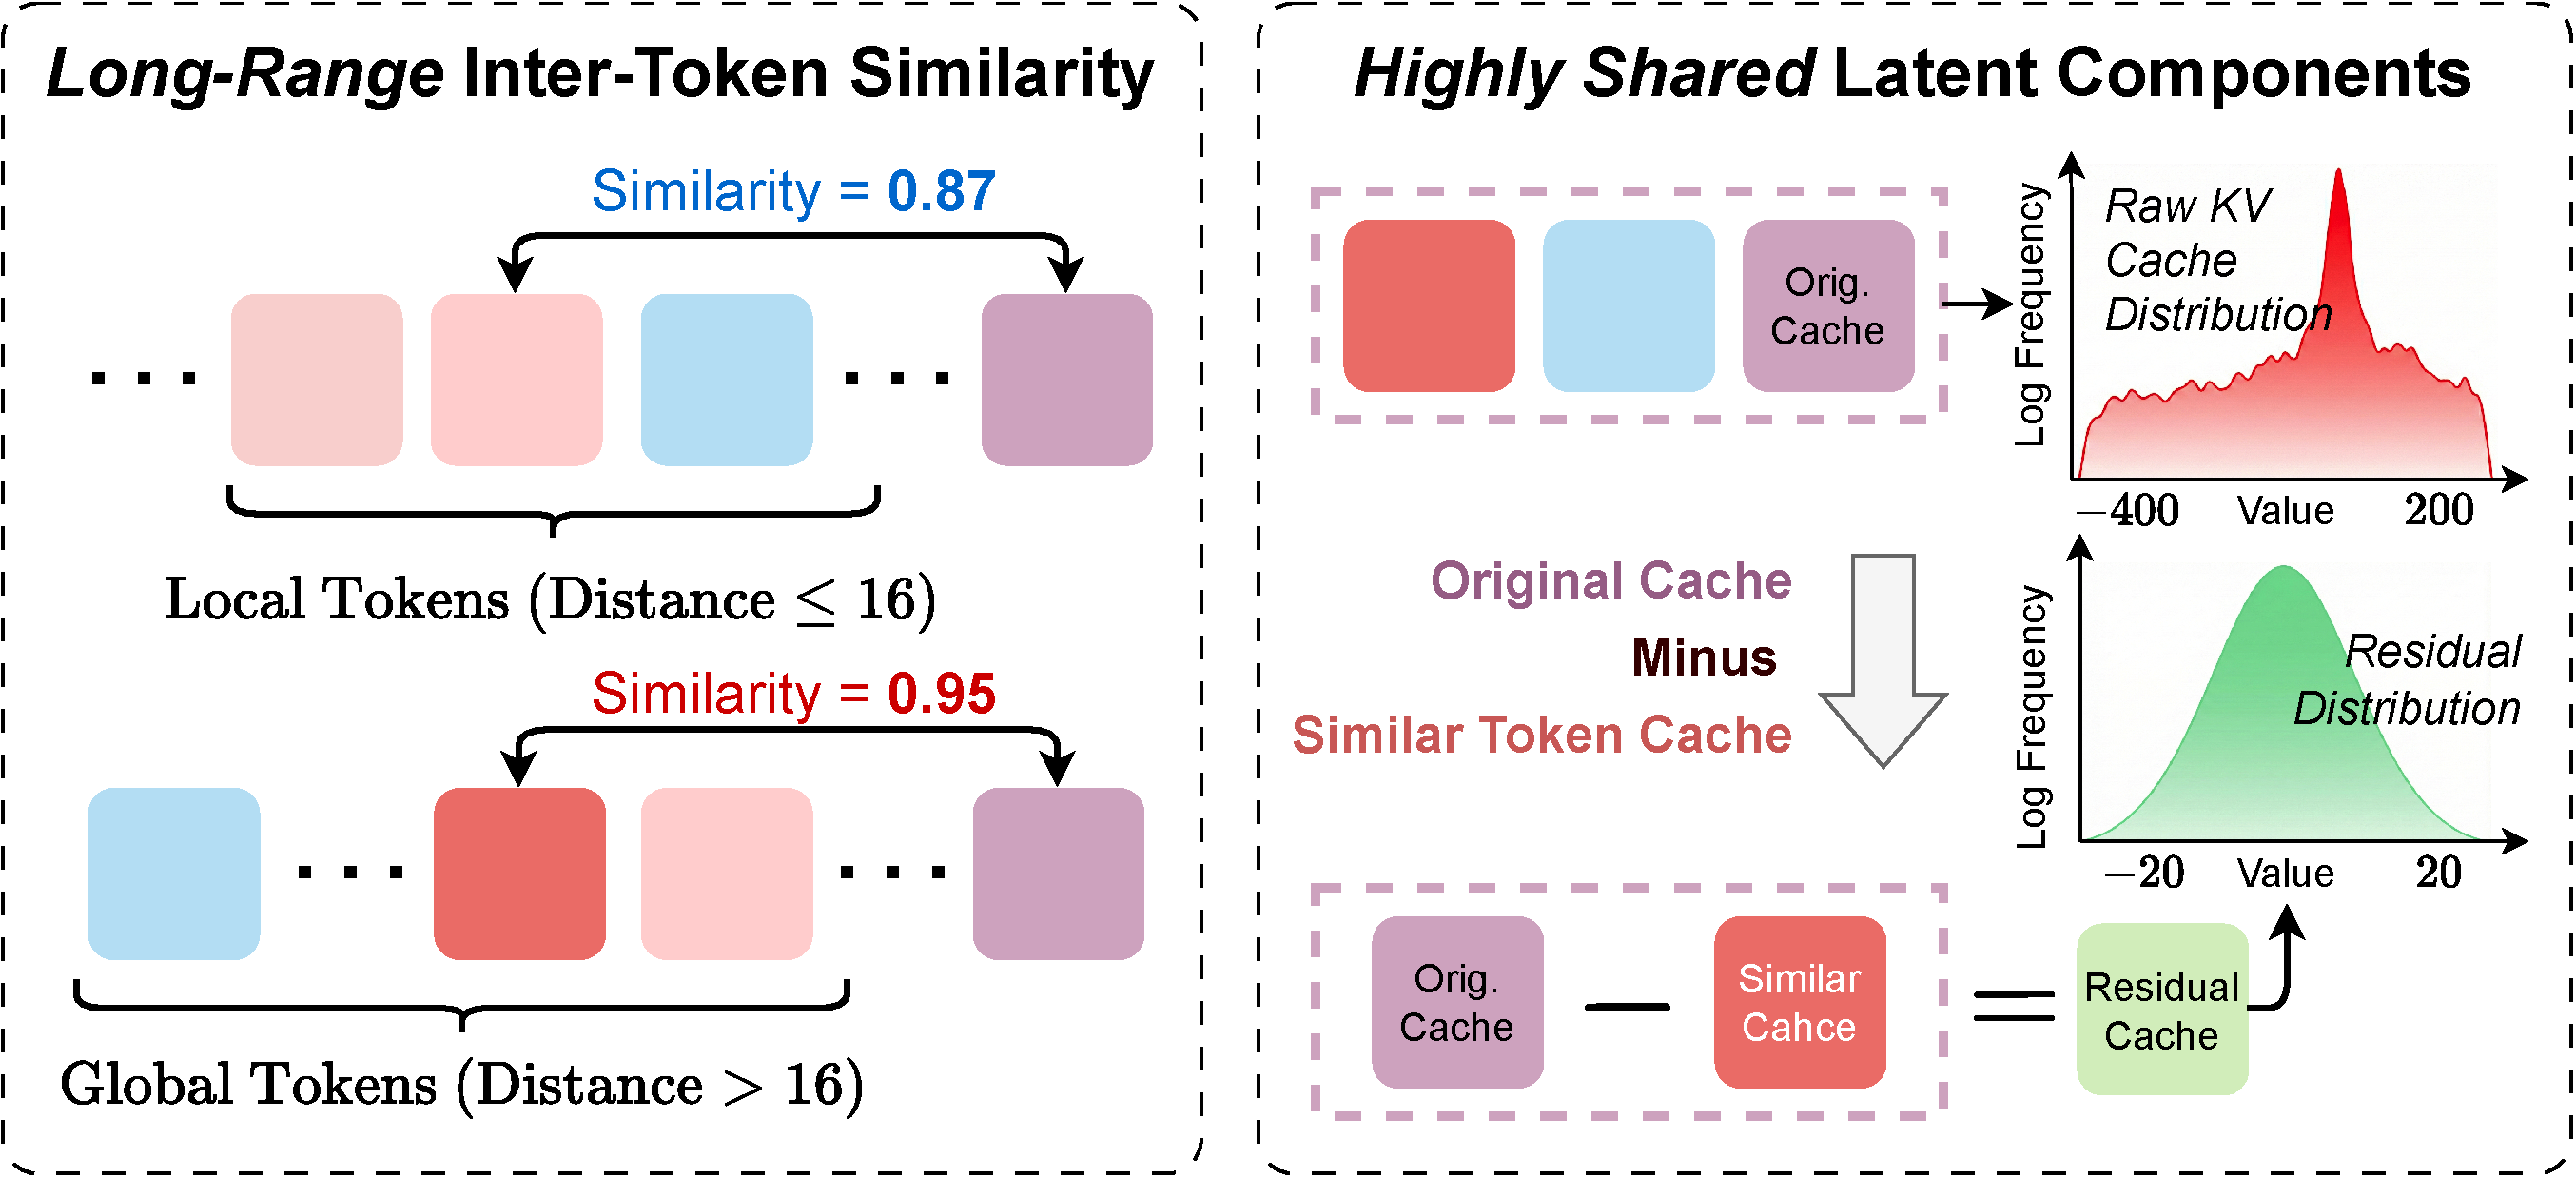
\includegraphics[width=0.99\columnwidth]{figures/DeltaKV-teaser.pdf} 
  \caption{\textbf{Illustration of two empirical observations in KV caches:} \emph{long-range} inter-token similarity beyond local context and \emph{highly shared} latent components across KV representations.}
  \label{fig:teaser}
  \vspace{-1.5em}
\end{figure}

Nevertheless, in realistic multi-stage settings where model focus shifts (e.g., multi-turn dialogue \cite{li2024scbench} and complex reasoning \cite{maa_aime}), static eviction methods like SnapKV often discard tokens that later become critical, causing large performance drops.
%%%
Dynamic sparsity methods (e.g., OmniKV, Quest) mitigate this by retaining the full KV cache and applying sparse attention, but they do not fundamentally reduce GPU memory without offloading, which introduces latency and PCIe overhead.

Beyond token selection, \textbf{KV cache compression} offers a more principled path toward memory reduction. 
%%%
Nonetheless, existing compression approaches face substantial obstacles when deployed in real systems, particularly in balancing compression effectiveness, hardware efficiency, and framework compatibility:
\begin{itemize}[nolistsep, left=0pt]
  \item \textbf{Local Similarity Bias:}
  Methods such as CacheGen \cite{liu2024cachegen} and Chelsea \cite{hu2025efficient_chelsea} exploit similarity among nearby tokens, but implicitly assume locality. 
  As we show in Figure \ref{fig:distance_dist_to_sim_tokens}, this assumption overlooks substantial \emph{global} similarity across distant tokens.
  
  \item \textbf{GPU-Unfriendly Pipeline:}
  Approaches like PQCache \cite{zhang2025pqcache} and Lexico~\cite{kim2024lexico} rely on multi-stage compression pipelines or complex codebooks, which introduce irregular memory access patterns, GPU underutilization, and reduced throughput.

  \item \textbf{Poor Integration with Inference Frameworks:} 
  Methods that evict tokens unevenly across layers (e.g., SnapKV) or impose heterogeneous per-layer/per-head budgets (e.g., PyramidKV \cite{cai2024pyramidkv} and AdaKV \cite{feng2025adakv}) are difficult to integrate into production-grade inference engines such as vLLM \cite{kwon2023efficient_vllm} and SGLang \cite{zheng2024sglang}. 
  As a result, many promising sparsity and compression techniques remain impractical in real deployments.
\end{itemize}

Motivated by these limitations, we conduct an empirical analysis of KV cache representations and uncover two key observations, illustrated in Figure~\ref{fig:teaser}:
\textbf{(1) \emph{Long-Range} Inter-Token Similarity:} Contrary to locality-driven assumptions, semantically similar tokens are often distributed \emph{globally} across the context rather than confined to nearby positions.
\textbf{(2) \emph{Highly Shared} Latent Components:} KV caches exhibit strong anisotropy, with a small number of high-norm latent directions capturing common linguistic and structural patterns shared across many tokens.
%%%
These observations indicate that much of the KV cache is redundant shared structure, while the remaining token-specific information is comparatively low-magnitude and easier to compress.

Based on this insight, we propose \textbf{DeltaKV}, a \emph{simple, residual-based, and GPU-friendly} KV cache compression framework that reduces KV cache memory to \textbf{29\%} of its original size while maintaining near-lossless performance.
%%%
DeltaKV partitions the KV cache into a small set of uncompressed reference tokens and a larger set of compressed tokens. 
For each compressed token, DeltaKV retrieves a few globally similar references, subtracts their shared components, and encodes only the resulting \emph{residual} using a lightweight MLP or linear projection.

During inference, DeltaKV naturally complements sparse attention methods such as OmniKV: only a small subset of important tokens are reconstructed on demand, avoiding unnecessary decompression and memory I/O.
%%%
Despite introducing compressor and decompressor modules, DeltaKV adds negligible parameter overhead (typically under $\mathbf{5\%}$ and can be trained efficiently in approximately $\mathbf{8}$ GPU hours.

\paragraph{Contributions}
Our contributions are threefold:
\begin{itemize}[nolistsep, left=0pt]
  \vspace{-0.5em}
  \item \textbf{Global Redundancy in KV Caches:}
  We show that KV cache similarity is fundamentally \emph{global}: over \textbf{60\%} of similar tokens are separated by more than \textbf{16 positions}. 
  We further identify dominant high-norm shared components whose removal yields low-magnitude residuals, exposing global redundancy (Figure~\ref{fig:combined_analysis_results}).
  
  \item \textbf{DeltaKV: Residual-Based, GPU-Friendly KV Cache Compression:} 
  We introduce DeltaKV, a residual-based KV cache compression framework that encodes only token-specific deviations from a small set of globally retrieved references. 
  DeltaKV uses lightweight linear or MLP projections, is fully GPU-friendly, and reduces KV cache memory to \textbf{29\%} with near-lossless accuracy.

  \item \textbf{Sparse-vLLM for Practical Deployment:}
  We present Sparse-vLLM, an inference framework for sparse and compressed KV caches with irregular memory layouts. 
  It supports DeltaKV and related methods and achieves up to $\mathbf{2}\times$ higher throughput than vLLM, enabling practical deployment of KV cache compression.
\end{itemize}


